% Source-derived connectivity. Generated by build_downstate_figure.py.%
% Display positions are schematic. CSVs preserve every represented bus and circuit key.%
\begingroup%
\definecolor{dsAdded}{RGB}{140,24,48}%
\definecolor{dsOld}{RGB}{113,118,122}%
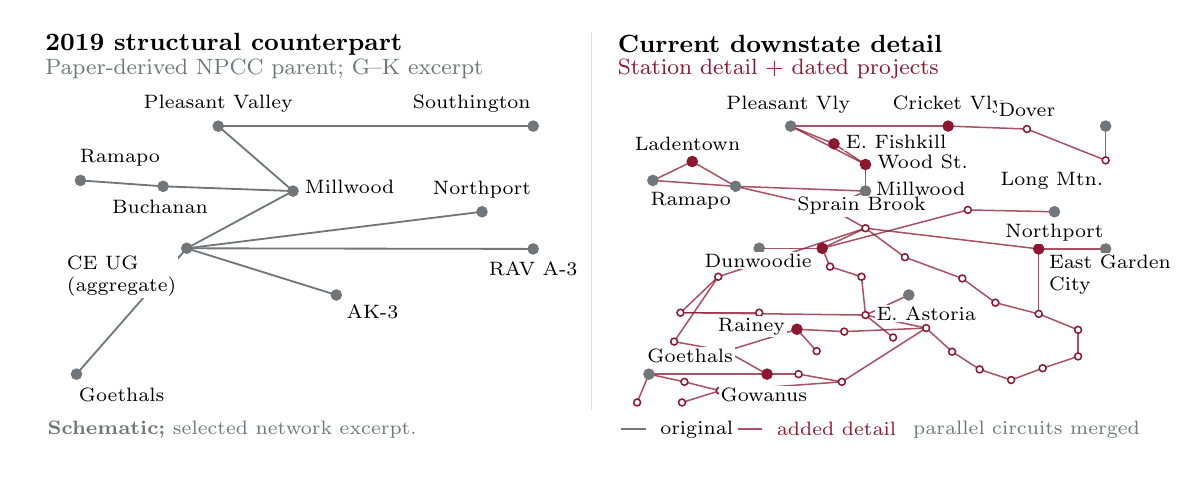
\begin{tikzpicture}[x=1cm,y=1cm, every node/.style={font=\fontsize{7.1}{8}\selectfont},%
 dsOriginal/.style={draw=dsOld,line width=.66pt},%
 dsAddedLine/.style={draw=dsAdded,line width=.55pt,opacity=.75},%
 dsLabel/.style={fill=white,inner sep=.7pt,text=black,align=left}]%
\path[use as bounding box] (0,0) rectangle (14.4,5.4);%
\node[anchor=west,font=\small\bfseries] at (.10,5.19) {2019 structural counterpart};%
\node[anchor=west,font=\small\bfseries] at (7.37,5.19) {Current downstate detail};%
\node[anchor=west,text=dsOld,font=\fontsize{8}{9}\selectfont] at (.10,4.88) {Paper-derived NPCC parent; G--K excerpt};%
\node[anchor=west,text=dsAdded,font=\fontsize{8}{9}\selectfont] at (7.37,4.88) {Station detail + dated projects};%
\draw[gray!25,line width=.4pt] (7.16,.54)--(7.16,5.35);%
% PARENT:32%
\draw[dsOriginal] (2.420,4.150) -- (6.420,4.150);%
% PARENT:87%
\draw[dsOriginal] (3.370,3.325) -- (2.420,4.150);%
% PARENT:88%
\draw[dsOriginal] (1.720,3.385) -- (3.370,3.325);%
% PARENT:89%
\draw[dsOriginal] (2.020,2.598) -- (3.370,3.325);%
% PARENT:91%
\draw[dsOriginal] (1.720,3.385) -- (0.670,3.460);%
% PARENT:92%
\draw[dsOriginal] (2.020,2.598) -- (6.420,2.590);%
% PARENT:93%
\draw[dsOriginal] (2.020,2.598) -- (5.770,3.062);%
% PARENT:94%
\draw[dsOriginal] (2.020,2.598) -- (0.620,1.000);%
% PARENT:95%
\draw[dsOriginal] (3.920,2.005) -- (2.020,2.598);%
\filldraw[draw=dsOld,fill=dsOld,line width=.55pt] (2.420,4.150) circle[radius=1.8pt];%
\filldraw[draw=dsOld,fill=dsOld,line width=.55pt] (0.670,3.460) circle[radius=1.8pt];%
\filldraw[draw=dsOld,fill=dsOld,line width=.55pt] (1.720,3.385) circle[radius=1.8pt];%
\filldraw[draw=dsOld,fill=dsOld,line width=.55pt] (3.370,3.325) circle[radius=1.8pt];%
\filldraw[draw=dsOld,fill=dsOld,line width=.55pt] (2.020,2.598) circle[radius=1.8pt];%
\filldraw[draw=dsOld,fill=dsOld,line width=.55pt] (6.420,2.590) circle[radius=1.8pt];%
\filldraw[draw=dsOld,fill=dsOld,line width=.55pt] (5.770,3.062) circle[radius=1.8pt];%
\filldraw[draw=dsOld,fill=dsOld,line width=.55pt] (0.620,1.000) circle[radius=1.8pt];%
\filldraw[draw=dsOld,fill=dsOld,line width=.55pt] (3.920,2.005) circle[radius=1.8pt];%
\filldraw[draw=dsOld,fill=dsOld,line width=.55pt] (6.420,4.150) circle[radius=1.8pt];%
% PERFORM:210, PERFORM:211%
\draw[dsAddedLine] (10.640,1.750) -- (8.290,1.780);%
% PERFORM:212, PERFORM:213%
\draw[dsAddedLine] (8.290,1.780) -- (8.770,2.237);%
% PERFORM:1107, PERFORM:1108, PERFORM:1109, PERFORM:1110%
\draw[dsAddedLine] (10.640,2.853) -- (10.190,3.107);%
% PERFORM:1111, PERFORM:1112, PERFORM:1113%
\draw[dsAddedLine] (10.640,3.325) -- (10.190,3.107);%
% PERFORM:1114%
\draw[dsAddedLine] (8.990,3.385) -- (10.190,3.107);%
% PERFORM:1159%
\draw[dsAddedLine] (10.090,2.598) -- (11.940,3.085);%
% PERFORM:1162%
\draw[dsAddedLine] (12.290,1.907) -- (12.840,1.765);%
% PERFORM:1164%
\draw[dsAddedLine] (11.870,2.215) -- (12.290,1.907);%
% PERFORM:1172, PERFORM:1173%
\draw[dsAddedLine] (12.840,1.765) -- (13.340,1.562);%
% PERFORM:1174, PERFORM:1175%
\draw[dsAddedLine] (12.840,2.590) -- (12.840,1.765);%
% PERFORM:1212, PERFORM:1213%
\draw[dsAddedLine] (13.340,1.225) -- (13.340,1.562);%
% PERFORM:1214, PERFORM:1215%
\draw[dsAddedLine] (12.840,2.590) -- (10.640,2.853);%
% PERFORM:1226, PERFORM:1227, PERFORM:1228, PERFORM:1229%
\draw[dsAddedLine] (10.090,2.598) -- (10.640,2.853);%
% PERFORM:1236, PERFORM:1237%
\draw[dsAddedLine] (10.640,2.853) -- (8.770,2.237);%
% PERFORM:1241, PERFORM:1242, PERFORM:1243%
\draw[dsAddedLine] (10.590,2.237) -- (10.190,2.365);%
% PERFORM:1245%
\draw[dsAddedLine] (10.640,1.750) -- (10.590,2.237);%
% PERFORM:1248, PERFORM:1249, PERFORM:1250%
\draw[dsAddedLine] (10.640,2.853) -- (11.140,2.485);%
% PERFORM:1257, PERFORM:1258%
\draw[dsAddedLine] (10.640,1.750) -- (10.990,1.465);%
% PERFORM:1260%
\draw[dsAddedLine] (11.870,2.215) -- (11.140,2.485);%
% PERFORM:1262, PERFORM:1263, PERFORM:1264%
\draw[dsAddedLine] (10.090,2.598) -- (10.190,2.365);%
% PERFORM:1265, PERFORM:1266, PERFORM:1267%
\draw[dsAddedLine] (11.410,1.585) -- (11.740,1.285);%
% PERFORM:1269, PERFORM:1270, PERFORM:1271, PERFORM:1272%
\draw[dsAddedLine] (10.640,1.750) -- (11.410,1.585);%
% PERFORM:1320, PERFORM:1321%
\draw[dsAddedLine] (12.490,0.925) -- (12.090,1.060);%
% PERFORM:1322, PERFORM:1323%
\draw[dsAddedLine] (12.490,0.925) -- (12.890,1.075);%
% PERFORM:1336, PERFORM:1337%
\draw[dsAddedLine] (11.740,1.285) -- (12.090,1.060);%
% PERFORM:1389, PERFORM:1390%
\draw[dsAddedLine] (10.240,3.925) -- (9.690,4.150);%
% PERFORM:1391, PERFORM:1392%
\draw[dsAddedLine] (9.690,4.150) -- (10.640,3.662);%
% PERFORM:1576%
\draw[dsAddedLine] (8.990,3.385) -- (8.440,3.700);%
% PERFORM:1577%
\draw[dsAddedLine] (8.440,3.700) -- (7.940,3.460);%
% PERFORM:1689, PERFORM:1690%
\draw[dsAddedLine] (10.240,3.925) -- (10.640,3.662);%
% PERFORM:1731, PERFORM:1732, PERFORM:1733%
\draw[dsAddedLine] (8.990,3.385) -- (10.640,3.325);%
% PERFORM:1734, PERFORM:1735%
\draw[dsAddedLine] (10.640,3.325) -- (10.640,3.662);%
% PERFORM:1738%
\draw[dsAddedLine] (8.990,3.385) -- (7.940,3.460);%
% PERFORM:1843, PERFORM:1844%
\draw[dsAddedLine] (12.890,1.075) -- (13.340,1.225);%
% PERFORM:1984, PERFORM:1985%
\draw[dsAddedLine] (8.870,1.292) -- (9.390,1.000);%
% PERFORM:1988, PERFORM:1989%
\draw[dsAddedLine] (8.870,1.292) -- (9.770,1.570);%
% PERFORM:1994%
\draw[dsAddedLine] (8.870,1.292) -- (8.210,1.413);%
% PERFORM:1997, PERFORM:1998, PERFORM:1999%
\draw[dsAddedLine] (9.770,1.570) -- (10.020,1.292);%
% PERFORM:2000%
\draw[dsAddedLine] (8.210,1.413) -- (8.770,2.237);%
% ATTACH:CEUG_DUNWOODIE%
\draw[dsAddedLine] (9.290,2.598) -- (10.090,2.598);%
% ATTACH:RAVA3_EGC%
\draw[dsAddedLine] (12.840,2.590) -- (13.690,2.590);%
% ATTACH:NORTHPORT_SHORERD%
\draw[dsAddedLine] (13.040,3.062) -- (11.940,3.085);%
% ATTACH:GOETHALS_GOWANUS%
\draw[dsAddedLine] (7.890,1.000) -- (9.390,1.000);%
% ATTACH:AK3_ASTORIA138%
\draw[dsAddedLine] (11.190,2.005) -- (10.640,1.750);%
% CV:BOUNDARY_SOUTHINGTON_LM%
\draw[dsAddedLine] (13.690,3.715) -- (13.690,4.150);%
% CV:PV_CV_F83_PROXY, CV:PV_CV_F84%
\draw[dsAddedLine] (11.690,4.150) -- (9.690,4.150);%
% DOVER:CV_DOVER_Y17%
\draw[dsAddedLine] (11.690,4.150) -- (12.690,4.113);%
% RECEIVING:GREENWOOD_CORONA%
\draw[dsAddedLine] (11.410,1.585) -- (10.340,0.902);%
% RECEIVING:FOXHILLS_GREENWOOD%
\draw[dsAddedLine] (8.790,0.790) -- (10.340,0.902);%
% ASSET:ANNEX_E13_Q35_PROXY%
\draw[dsAddedLine] (9.290,1.780) -- (8.290,1.780);%
% ASSET:FRESHKILLS138_FOXHILLS%
\draw[dsAddedLine] (8.310,0.640) -- (8.790,0.790);%
% ASSET:FRESHKILLS345_GOETHALS%
\draw[dsAddedLine] (7.740,0.640) -- (7.890,1.000);%
% RCC:PAR:GOWANUS%
\draw[dsAddedLine] (9.390,1.000) -- (9.790,1.000);%
% RCC:PAR:GOETHALS%
\draw[dsAddedLine] (7.890,1.000) -- (8.340,0.902);%
% RCC:PAR:RAINEY%
\draw[dsAddedLine] (9.770,1.570) -- (10.370,1.540);%
% RCC:CABLE:QUEENS%
\draw[dsAddedLine] (11.410,1.585) -- (10.370,1.540);%
% RCC:CABLE:BROOKLYN%
\draw[dsAddedLine] (10.340,0.902) -- (9.790,1.000);%
% RCC:CABLE:STATEN%
\draw[dsAddedLine] (8.790,0.790) -- (8.340,0.902);%
% DOVER:RESOLVED_398%
\draw[dsAddedLine] (12.690,4.113) -- (13.690,3.715);%
\filldraw[draw=dsOld,fill=dsOld,line width=.55pt] (9.690,4.150) circle[radius=1.8pt];%
\filldraw[draw=dsOld,fill=dsOld,line width=.55pt] (7.940,3.460) circle[radius=1.8pt];%
\filldraw[draw=dsOld,fill=dsOld,line width=.55pt] (8.990,3.385) circle[radius=1.8pt];%
\filldraw[draw=dsOld,fill=dsOld,line width=.55pt] (10.640,3.325) circle[radius=1.8pt];%
\filldraw[draw=dsOld,fill=dsOld,line width=.55pt] (9.290,2.598) circle[radius=1.8pt];%
\filldraw[draw=dsOld,fill=dsOld,line width=.55pt] (13.690,2.590) circle[radius=1.8pt];%
\filldraw[draw=dsOld,fill=dsOld,line width=.55pt] (13.040,3.062) circle[radius=1.8pt];%
\filldraw[draw=dsOld,fill=dsOld,line width=.55pt] (7.890,1.000) circle[radius=1.8pt];%
\filldraw[draw=dsOld,fill=dsOld,line width=.55pt] (11.190,2.005) circle[radius=1.8pt];%
\filldraw[draw=dsAdded,fill=dsAdded,line width=.55pt] (10.240,3.925) circle[radius=1.8pt];%
\filldraw[draw=dsAdded,fill=dsAdded,line width=.55pt] (10.640,3.662) circle[radius=1.8pt];%
\filldraw[draw=dsAdded,fill=dsAdded,line width=.55pt] (8.440,3.700) circle[radius=1.8pt];%
\filldraw[draw=dsAdded,fill=dsAdded,line width=.55pt] (11.690,4.150) circle[radius=1.8pt];%
\filldraw[draw=dsAdded,fill=white,line width=.55pt] (12.690,4.113) circle[radius=1.25pt];%
\filldraw[draw=dsAdded,fill=white,line width=.55pt] (13.690,3.715) circle[radius=1.25pt];%
\filldraw[draw=dsOld,fill=dsOld,line width=.55pt] (13.690,4.150) circle[radius=1.8pt];%
\filldraw[draw=dsAdded,fill=white,line width=.55pt] (10.190,3.107) circle[radius=1.25pt];%
\filldraw[draw=dsAdded,fill=white,line width=.55pt] (10.640,2.853) circle[radius=1.25pt];%
\filldraw[draw=dsAdded,fill=dsAdded,line width=.55pt] (10.090,2.598) circle[radius=1.8pt];%
\filldraw[draw=dsAdded,fill=white,line width=.55pt] (11.940,3.085) circle[radius=1.25pt];%
\filldraw[draw=dsAdded,fill=dsAdded,line width=.55pt] (12.840,2.590) circle[radius=1.8pt];%
\filldraw[draw=dsAdded,fill=white,line width=.55pt] (11.870,2.215) circle[radius=1.25pt];%
\filldraw[draw=dsAdded,fill=white,line width=.55pt] (12.290,1.907) circle[radius=1.25pt];%
\filldraw[draw=dsAdded,fill=white,line width=.55pt] (12.840,1.765) circle[radius=1.25pt];%
\filldraw[draw=dsAdded,fill=white,line width=.55pt] (13.340,1.562) circle[radius=1.25pt];%
\filldraw[draw=dsAdded,fill=white,line width=.55pt] (13.340,1.225) circle[radius=1.25pt];%
\filldraw[draw=dsAdded,fill=white,line width=.55pt] (12.890,1.075) circle[radius=1.25pt];%
\filldraw[draw=dsAdded,fill=white,line width=.55pt] (12.490,0.925) circle[radius=1.25pt];%
\filldraw[draw=dsAdded,fill=white,line width=.55pt] (12.090,1.060) circle[radius=1.25pt];%
\filldraw[draw=dsAdded,fill=white,line width=.55pt] (10.190,2.365) circle[radius=1.25pt];%
\filldraw[draw=dsAdded,fill=white,line width=.55pt] (10.590,2.237) circle[radius=1.25pt];%
\filldraw[draw=dsAdded,fill=white,line width=.55pt] (11.140,2.485) circle[radius=1.25pt];%
\filldraw[draw=dsAdded,fill=white,line width=.55pt] (10.640,1.750) circle[radius=1.25pt];%
\filldraw[draw=dsAdded,fill=white,line width=.55pt] (10.990,1.465) circle[radius=1.25pt];%
\filldraw[draw=dsAdded,fill=white,line width=.55pt] (11.410,1.585) circle[radius=1.25pt];%
\filldraw[draw=dsAdded,fill=white,line width=.55pt] (11.740,1.285) circle[radius=1.25pt];%
\filldraw[draw=dsAdded,fill=white,line width=.55pt] (8.770,2.237) circle[radius=1.25pt];%
\filldraw[draw=dsAdded,fill=white,line width=.55pt] (8.290,1.780) circle[radius=1.25pt];%
\filldraw[draw=dsAdded,fill=white,line width=.55pt] (8.210,1.413) circle[radius=1.25pt];%
\filldraw[draw=dsAdded,fill=white,line width=.55pt] (8.870,1.292) circle[radius=1.25pt];%
\filldraw[draw=dsAdded,fill=dsAdded,line width=.55pt] (9.390,1.000) circle[radius=1.8pt];%
\filldraw[draw=dsAdded,fill=dsAdded,line width=.55pt] (9.770,1.570) circle[radius=1.8pt];%
\filldraw[draw=dsAdded,fill=white,line width=.55pt] (10.020,1.292) circle[radius=1.25pt];%
\filldraw[draw=dsAdded,fill=white,line width=.55pt] (10.370,1.540) circle[radius=1.25pt];%
\filldraw[draw=dsAdded,fill=white,line width=.55pt] (9.790,1.000) circle[radius=1.25pt];%
\filldraw[draw=dsAdded,fill=white,line width=.55pt] (8.340,0.902) circle[radius=1.25pt];%
\filldraw[draw=dsAdded,fill=white,line width=.55pt] (10.340,0.902) circle[radius=1.25pt];%
\filldraw[draw=dsAdded,fill=white,line width=.55pt] (8.790,0.790) circle[radius=1.25pt];%
\filldraw[draw=dsAdded,fill=white,line width=.55pt] (8.310,0.640) circle[radius=1.25pt];%
\filldraw[draw=dsAdded,fill=white,line width=.55pt] (7.740,0.640) circle[radius=1.25pt];%
\filldraw[draw=dsAdded,fill=white,line width=.55pt] (9.290,1.780) circle[radius=1.25pt];%
\node[dsLabel,anchor=south,text=black] at (2.420,4.290) {Pleasant Valley};%
\node[dsLabel,anchor=south west,text=black] at (0.630,3.610) {Ramapo};%
\node[dsLabel,anchor=north,text=black] at (1.680,3.245) {Buchanan};%
\node[dsLabel,anchor=west,text=black] at (3.490,3.385) {Millwood};%
\node[dsLabel,anchor=north east,text=black] at (1.920,2.528) {CE UG\\(aggregate)};%
\node[dsLabel,anchor=north,text=black] at (6.420,2.450) {RAV A-3};%
\node[dsLabel,anchor=south,text=black] at (5.770,3.203) {Northport};%
\node[dsLabel,anchor=north west,text=black] at (0.620,0.860) {Goethals};%
\node[dsLabel,anchor=north west,text=black] at (4.020,1.905) {AK-3};%
\node[dsLabel,anchor=south east,text=black] at (6.420,4.290) {Southington};%
\node[dsLabel,anchor=south,text=black] at (9.660,4.280) {Pleasant Vly};%
\node[dsLabel,anchor=north west,text=black] at (7.880,3.340) {Ramapo};%
\node[dsLabel,anchor=west,text=black] at (10.740,3.355) {Millwood};%
\node[dsLabel,anchor=west,text=black] at (10.360,3.945) {E. Fishkill};%
\node[dsLabel,anchor=west,text=black] at (10.760,3.702) {Wood St.};%
\node[dsLabel,anchor=south,text=black] at (8.380,3.810) {Ladentown};%
\node[dsLabel,anchor=south,text=black] at (11.690,4.280) {Cricket Vly};%
\node[dsLabel,anchor=south,text=black] at (12.690,4.243) {Dover};%
\node[dsLabel,anchor=north east,text=black] at (13.690,3.595) {Long Mtn.};%
\node[dsLabel,anchor=south,text=black] at (10.590,2.993) {Sprain Brook};%
\node[dsLabel,anchor=north east,text=black] at (9.990,2.558) {Dunwoodie};%
\node[dsLabel,anchor=north west,text=black] at (12.940,2.550) {East Garden\\City};%
\node[dsLabel,anchor=north,text=black] at (13.040,2.933) {Northport};%
\node[dsLabel,anchor=west,text=black] at (10.750,1.770) {E. Astoria};%
\node[dsLabel,anchor=east,text=black] at (9.650,1.600) {Rainey};%
\node[dsLabel,anchor=north,text=black] at (9.350,0.850) {Gowanus};%
\node[dsLabel,anchor=south west,text=black] at (7.840,1.120) {Goethals};%
\node[anchor=west,text=dsOld,font=\fontsize{7.5}{8.5}\selectfont] at (.13,.30) {\textbf{Schematic;} selected network excerpt.};%
\draw[dsOriginal] (7.54,.30)--(7.85,.30);%
\node[anchor=west] at (7.91,.30) {original};%
\draw[dsAddedLine] (9.02,.30)--(9.33,.30);%
\node[anchor=west,text=dsAdded] at (9.39,.30) {added detail};%
\node[anchor=east,text=dsOld,font=\fontsize{7.1}{8}\selectfont] at (14.25,.30) {parallel circuits merged};%
\end{tikzpicture}%
\endgroup%
